\section{Introduction}

\begin{figure}[t]
    \centering
    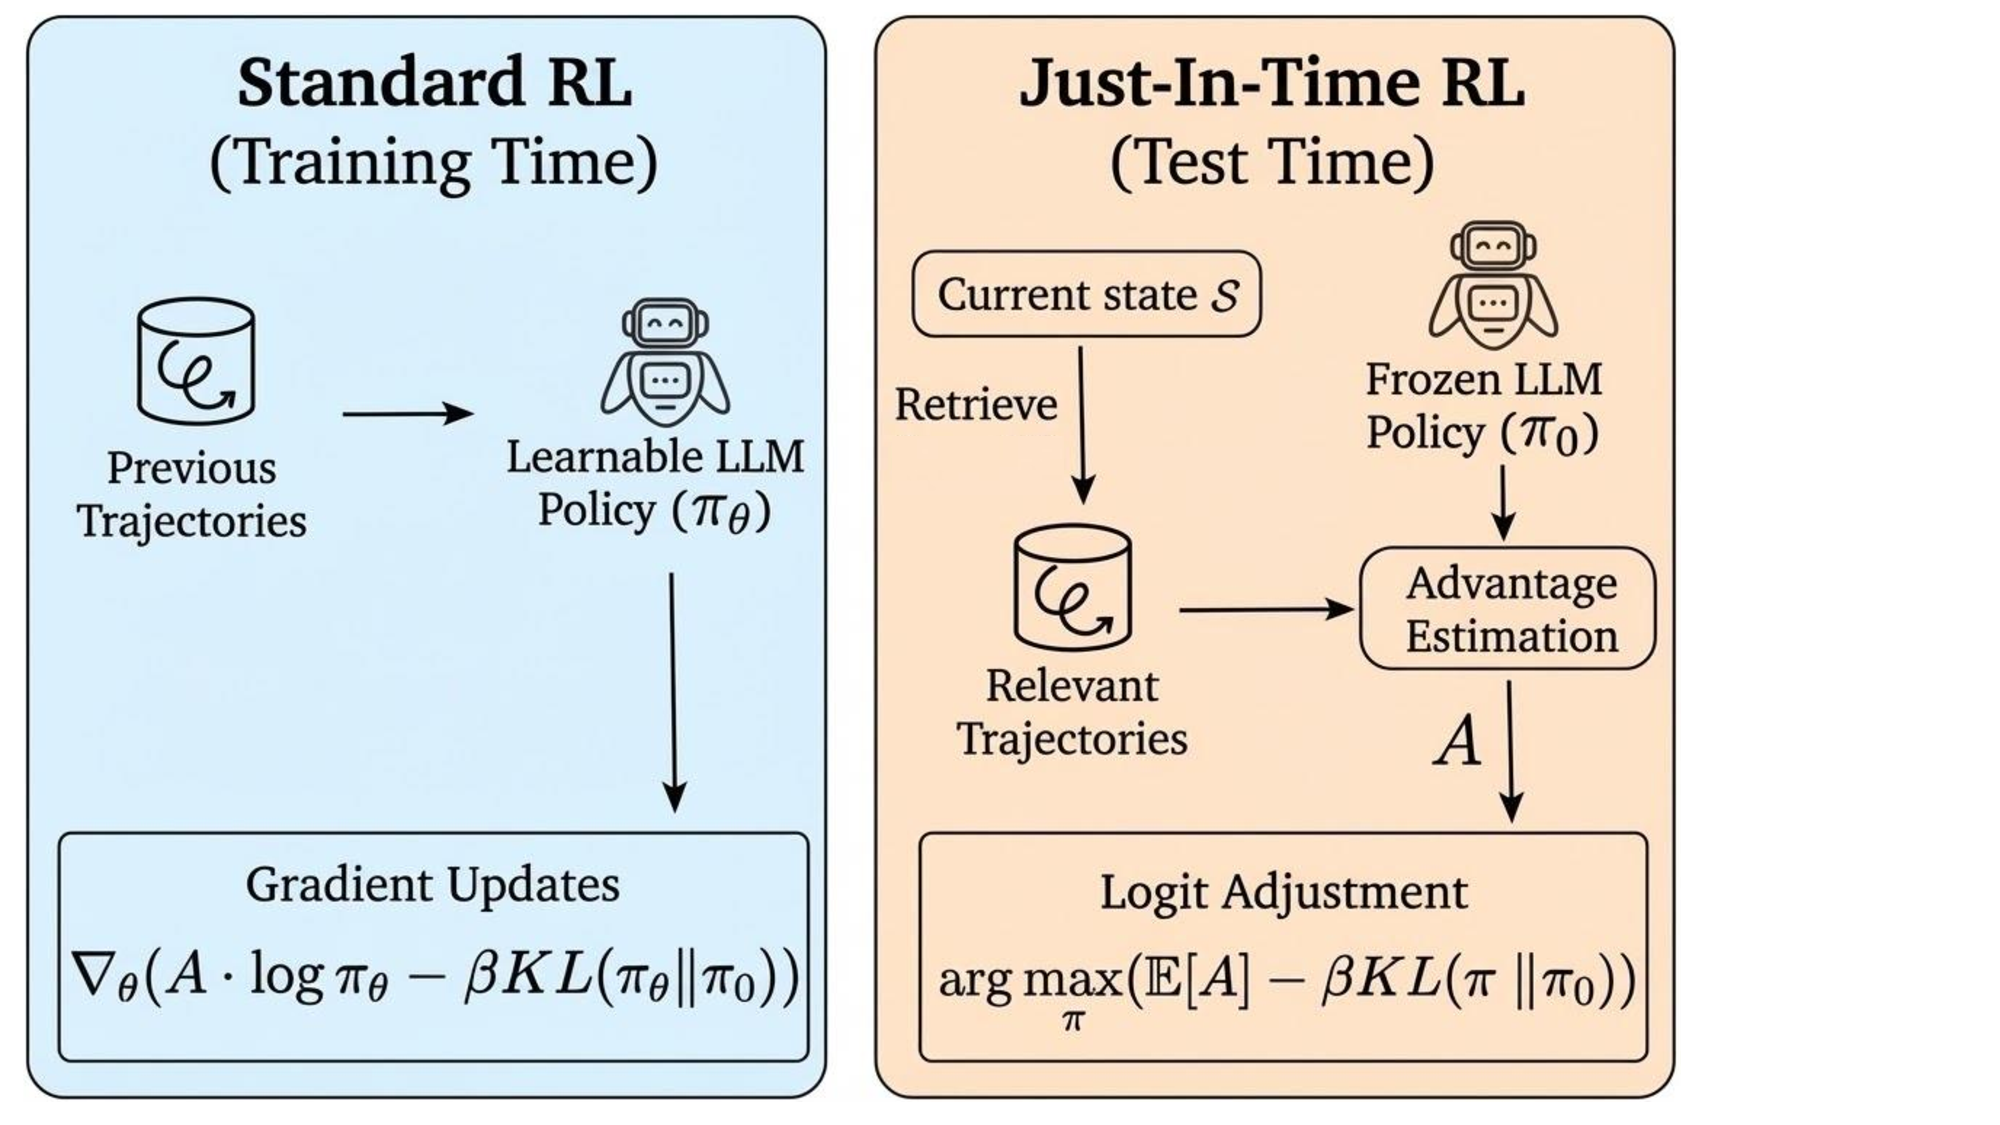
\includegraphics[width=\linewidth]{figures/TestRL.pdf}
    \caption{While standard RL performs policy gradient updates during training using previous trajectories, JitRL operates at test time. Specifically, it retrieves trajectories relevant to the current state to estimate advantages $A$, subsequently refining the output logits through a KL-regularized policy optimization objective.}
    \label{fig:intro}
\end{figure}



While humans can learn ``on the fly'', current AI agents fundamentally lack this ability because their weights are frozen after training \citep{self-evolving, self-evolving2, conftuner}. This limitation severely restricts their practicality: when deployed in unfamiliar or dynamic settings, AI agents are analogous to newly hired employees without on-the-job training, which often repeatedly make the same errors due to their failure to learn, whereas humans can adapt to their environment, including by learning from their mistakes. Highlighting the importance of this issue, \citet{hendrycks2025definition} proposes an “AGI Score” assessing progress toward artificial general intelligence and finds that current AI systems are most deficient in their “capability to continually learn new information”.

One potential solution is conventional reinforcement learning (RL) \citep{webrl,toolrl,torl}, performed in a continually policy gradient updating manner. However, this approach requires a large amount of training data to perform well. It is also computationally expensive, due to the high cost of RL and the need for frequent updates to keep the model up to date. In addition, it is prone to catastrophic forgetting, degrading the model’s previously learned capabilities \citep{catastrophic}. Prior work finds that conventional RL yields only limited improvements when evaluated in continual adaptation settings \cite{evotest}.

An alternative approach to this problem relies on in-context learning (ICL) \citep{icl} to enable the agent to learn at test time \citep{reflexion,awm}. These methods rely on prompt or context engineering to incorporate information from past experiences. However, such approaches tend to struggle as the required context length grows, especially since agentic tasks often involve long sequences of interactions \cite{lost-in-the-middle}. Crucially, ICL lacks the generality of RL. While prompts are confined to explicit textual descriptions, RL optimizes policies through rewards, enabling the mastery of complex skills that are difficult to articulate in text.

In light of these limitations, a fundamental question arises: \textit{Can we enable agents to learn continually in a flexible way, without expensive parameter updates?} Our approach, Just-In-Time Reinforcement Learning (JitRL), enables general-purpose learning by adopting an RL formulation, while maintaining efficiency by avoiding gradient updates. Instead of gradient updates, JitRL maintains a dynamic memory bank that stores trajectories as \texttt{<state, action, reward>} triplets, as illustrated in Figure ~\ref{fig:intro}. Then, given the agent's current state, it retrieves relevant trajectories from the memory, and learns from them ``just in time.'' To do so, it uses these trajectories to estimate the advantage of each action in the current state -- i.e., how much better each action is relative to the average. These advantage estimates are then used to adjust the model's output logits. Crucially, we theoretically prove that our update rule is the exact closed-form solution to the policy optimization objective under a KL constraint. In this way, JitRL enables continual self-evolution without the prohibitive costs of gradient-based training. 

% We empirically validate...}



% Large Language Models (LLMs) have demonstrated exceptional capabilities across a wide spectrum of tasks. Furthermore, agents are used to solve tasks requiring domain-specific knowledge and long-horizon planning, such as navigating the web \cite{awm, mind2web}, operating mobile apps \citep{operating1, operating2}, and playing games \citep{evotest,game}. 


% Large Language Model agents are capable of executing long-horizon tasks, such as navigating the web \cite{awm, mind2web}, operating mobile apps \citep{operating1, operating2}, and playing games \citep{evotest,game}. However, while the environments are dynamic and evolving, the agents themselves are typically frozen after training. Consequently, they often repeat the same errors and fail to adapt to new scenarios, as they lack the ability to learn from their own past experiences.

% % Despite these advancements, they still cannot learn from past experiences and adapt to new, evolving environments.
% % Recent research has integrated Reinforcement Learning (RL) into the agentic loop. Methods like Group Relative Policy Optimization (GRPO) ~\citep{grpo} have shown promise in optimizing agent policies through environmental interaction. Despite their potential, gradient-based methods suffer from three critical limitations: (1) Prohibitive Compute: The memory and latency costs of on-policy updates are incompatible with large-scale LLM deployment; (2) Sparse Feedback: Relying on episodic rewards hinders precise, step-level policy refinement; and (3) Static Inference: The frozen nature of trained models precludes test-time adaptation, leaving agents vulnerable to distribution shifts and unable to learn from immediate interactions.

% To address this lack of adaptability, recent studies \citep{webrl} have utilized Reinforcement Learning (RL) to train agents through environmental interaction. While these gradient-based approaches have shown promise, they face three critical barriers to scalable deployment. First, standard RL algorithms often require a large amount of training samples to converge, which translates to prohibitive time and monetary costs. Second, performing on-policy gradient updates for large-scale models (e.g., 70B parameters) incurs substantial GPU resources, which are often inaccessible for typical deployment setups. Third, traditional training yields a static model, leaving it vulnerable to distribution shifts and unable to leverage immediate feedback from its current interactions.


% In light of these limitations, a fundamental question arises: \textit{Can we enable an agent to improve its policy continuously at test-time, bypassing the need for expensive parameter updates?}
% Realizing this vision, however, presents significant challenges. 
% First, how can we guarantee policy improvement when the model weights are frozen? Simple prompting-based methods lacks the mathematical guarantee of monotonic improvement found in gradient-based methods.
% Second, how do we perform efficient credit assignment in sparse-reward environments? Without a trainable value network, the agent struggles to assess intermediate steps, making it difficult to distinguish pivotal decisions from irrelevant actions.

% To bridge this gap, we propose a novel \textbf{Just-In-Time Reinforcement Learning (JitRL)}, a training-free framework that enables frozen LLMs to optimize their policy purely at test time. Instead of updating parameters, JitRL maintains a dynamic, non-parametric knowledge base that continually stores experience trajectories as \texttt{<state, action, reward>} triplets. During inference, it retrieves and aggregates relevant experiences to estimate action values, and directly updates the output logits based on these estimates. 
% Crucially, we theoretically prove that this additive update rule is the exact closed-form solution to the policy optimization objective under a KL constraint.
% This method effectively enables continuous self-evolution without the prohibitive costs of gradient-based training. 

We empirically validate JitRL on two benchmarks: WebArena \citep{webarena} for realistic web navigation and Jericho \citep{jericho} for long-horizon text-based games. Extensive experiments demonstrate that JitRL sets a new state-of-the-art,  outperforming training-free baselines and weight-update methods, while reducing the monetary costs of conventional RL by over 30×. Furthermore, our results highlight JitRL's robustness, showing consistent gains across diverse LLM backbones and effective generalization to unseen tasks. 

% Our contributions are summarized as follows:
% \begin{itemize}
%     \item \textbf{Framework:} We introduce Just-In-Time Reinforcement Learning (JitRL), enabling agents to continuously optimize strategies without gradient updates.
%     \item \textbf{Theory:} We theoretically prove that our JitRL is the exact closed-form solution to the reinforcement learning objective.
%     \item \textbf{Experiments:} Extensive evaluations demonstrate that JitRL significantly surpasses  baselines.
% \end{itemize}